\documentclass{rapport}
\usepackage{lipsum}
\usepackage{graphicx}
\title{TAROT_MONNIER_POINGT_PLANCHENAULT} %Titre du fichier

\begin{document}

%----------- Informations du rapport ---------

\logo{IMAGES/Logo Esiea - noir.png}
\titre{Rapport MLChallenge} %Titre du fichier .pdf
\cours{Machine Learning Challenge} %Nom du cours

\enseignant{Thibault \textsc{GEOFFROY}} %Nom de l'enseignant

\eleves{Bastien \textsc{TAROT} \\
    Raphael \textsc{MONNIER} \\
    Tanguy \textsc{POINGT} \\
    Allan \textsc{PLANCHENAULT} } %Nom des élèves

%----------- Initialisation -------------------

\fairemarges %Afficher les marges
\fairepagedegarde %Créer la page de garde
\tabledematieres %Créer la table de matières

%------------ Corps du rapport ----------------

\section{Introduction}

La reconnaissance des émotions est un domaine en pleine expansion qui suscite l'intérêt de
nombreux chercheurs en raison des défis complexes qu'il pose.
Malgré les avancées réalisées, ce problème reste encore partiellement résolu.
Ce champ d'étude est vaste, mais pour ce projet, nous nous concentrerons sur les émotions dites de base selon le modèle d'Ekman :
la joie, la colère, le dégoût, la tristesse, la peur et la surprise, en ajoutant également l'absence d'émotion,
c'est-à-dire l'état « neutre ».\\

\subsection{Objectifs du Projet}
Pour développer un système de reconnaissance des émotions en utilisant une approche de machine learning,
il est généralement recommandé de suivre un pipeline structuré. Dans le cadre de ce projet, apres la mise en place
des différents sujets d'introduction nous aborderons les grands thèmes suivants :\\

\textbf{Prétraitement et Extraction des Features :}
Les étapes nécessaires pour préparer les données et extraire les caractéristiques pertinentes pour la reconnaissance des émotions.\\

\textbf{Modèles Choisis :}
Les différents modèles de machine learning sélectionnés pour cette tâche et les raisons de leur choix.\\

\textbf{Évaluation des Modèles :}
Les méthodes et les métriques utilisées pour évaluer la performance des modèles de reconnaissance d émotions.\\

\textbf{Discussion des Résultats :}
Une analyse critique des résultats obtenus, mettant en évidence les points forts et les limitations des approches adoptées.\\

Cette structure permettra de couvrir de manière exhaustive les aspects clés du développement
d'un système de reconnaissance des émotions, de la préparation des données à l'évaluation des modèles.

\subsection{Etat de l'art}

L'une des premières étapes de ce challenge était de ce renseigner sur l'état
de l'art de la reconnaissance des émotions. Nous nous sommes majoritairement
intéressé à 3 articles que nous allons analyser dans les prochaine section.

\subsubsection{Analyse de l'article \cite{sariyanidiAutomaticAnalysisFacial2015} Automatic Analysis of Facial Affect: A Survey of Registration, Representation, and Recognition. L'auteur principal est Evangelos Sariyanidi.}

Dans l'article, les auteurs commencent par présenter l'objectif des systèmes de
reconnaissance des émotions, qui est d'identifier les actions faciales et les
émotions associées, notamment en se basant sur le Facial Action Coding System (FACS).
Le FACS code les expressions faciales en unités d'action (AUs) et distingue
les émotions basiques (comme la joie et la peur) et non-basiques. L'article
souligne aussi l'importance de l'évolution temporelle des expressions dans
l'interprétation des émotions et mentionne les défis liés à la reconnaissance des
émotions spontanées.\\

Les auteurs explique aussi à quel point l'enregistrement du visage joue un rôle
important dans la reconnaissance des émotions. Il existe trois stratégies
principales d'enregistrement du visage : l'enregistrement de l’ensemble du visage,
l’enregistrement de parties spécifiques, et l’enregistrement de points.
\begin{itemize}
    \item \textbf{Enregistrement du visage entier :} Ce type d’enregistrement peut être rigide ou
          non-rigide. Les approches rigides utilisent des points clés (comme les yeux,
          le nez ou la bouche) pour transformer le visage en fonction d’un modèle type.
          Les approches non-rigides, en revanche, permettent de déformer le visage, par
          exemple en transformant un visage expressif en un visage neutre, afin de minimiser
          les erreurs liées aux expressions faciales.
    \item \textbf{Enregistrement par parties :} Cette méthode divise le visage
          en différentes zones (comme les yeux et la bouche). Chaque partie
          est traitée indépendamment pour garantir une meilleure précision.
    \item \textbf{Enregistrement de points :} Utilisé pour les représentations
          basées sur la forme, ce type d'enregistrement localise des points
          précis sur le visage afin de suivre les changements de forme liés
          aux expressions.
\end{itemize}
Chaque méthode d'enregistrement a ses avantages et ses inconvénients, et le choix
de la technique dépend des objectifs du système de reconnaissance, notamment sa
capacité à gérer les variations de pose de tête et d'expressions naturelles.\\

La partie suivante de l'article traite des méthodes de représentation faciale.
Les auteurs classifient les représentations en deux grandes catégories : les
représentations spatiales et les représentations spatio-temporelles. Les
représentations spatiales analysent les images de manière indépendante, tandis que
les représentations spatio-temporelles prennent en compte une séquence d'images,
permettant ainsi de capturer les variations temporelles des expressions faciales.
Parmi les représentations spatiales, on trouve les représentations basées sur
l'apparence (comme les histogrammes des motifs locaux binaires - LBP - et les
transformées de Fourier locales - LPQ), ainsi que les représentations basées sur la
forme (qui décrivent les points caractéristiques du visage).\\

Ensuite, les auteurs examinent les techniques de réduction de la dimensionnalité
pour diminuer la complexité computationnelle tout en préservant les informations
pertinentes. Ces techniques incluent le pooling, qui regroupe les caractéristiques
locales et augmente la tolérance aux erreurs d'enregistrement. Le choix des
caractéristiques et l'extraction des caractéristiques (comme l'analyse en
composantes principales, PCA) sont aussi abordés pour améliorer les performances
des systèmes en réduisant la redondance des données.\\

Enfin, la section sur les modèles de reconnaissance explore les différentes
approches statistiques pour la reconnaissance des émotions. Les systèmes modernes
utilisent des techniques d'apprentissage automatique comme les machines à vecteurs
de support (SVM), les réseaux bayésiens dynamiques (DBN), et les modèles de champs
aléatoires conditionnels (CRF). Ces modèles permettent de modéliser les dépendances
temporelles et spatiales, et certains exploitent la personnalisation des modèles
pour s’adapter aux variations individuelles, comme les biais liés à l'identité.

\subsubsection{Analyse de l'article \cite{koBriefReviewFacial2018} A Brief Review of Facial Emotion Recognition Based on Visual Information. L'auteur est Byoung Chul Ko.}

Cet article présente un examen des méthodes de reconnaissance des émotions faciales
(FER) basées sur l'information visuelle, un sujet crucial dans les domaines de la
vision par ordinateur et de l'intelligence artificielle. La reconnaissance des
émotions faciales a des applications variées, notamment dans l'interaction
homme-machine, la réalité virtuelle, et les systèmes avancés d'assistance à la conduite.\\

L'article divise les approches en deux catégories principales : les méthodes classiques
et les méthodes basées sur l'apprentissage profond. Dans les approches classiques,
la reconnaissance des émotions se fait en trois étapes :
\begin{itemize}
    \item Détection des visages et des composants faciaux.
    \item Extraction des caractéristiques spatiales et temporelles à partir de ces composants.
    \item Classification des émotions à l'aide d'algorithmes comme les SVM (machines à vecteurs de support), AdaBoost, et Random Forest.
\end{itemize}
Ces méthodes reposent sur des caractéristiques définies manuellement, comme les
relations géométriques entre les composants faciaux ou les caractéristiques
d'apparence globale comme les histogrammes de motifs binaires locaux (LBP).
Cependant, elles présentent des limites face aux expressions spontanées et aux variations de pose.\\

Avec le développement des réseaux neuronaux profonds, l'apprentissage automatique
a radicalement amélioré la performance de la FER. Les réseaux de neurones convolutionnels
(CNN) sont largement utilisés pour extraire automatiquement des caractéristiques pertinentes
à partir d'images faciales. Ces modèles éliminent la dépendance à des modèles
basés sur la physique du visage, permettant une approche de bout en bout.
\\L'article décrit également des approches hybrides combinant des CNN pour les
caractéristiques spatiales et des réseaux de mémoire à long terme (LSTM) pour
capturer les dynamiques temporelles des expressions faciales dans les séquences vidéo.
Ces méthodes permettent de mieux modéliser les variations temporelles des expressions
faciales, offrant ainsi une meilleure performance dans la reconnaissance des émotions.\\

En conclusion, l'article souligne que bien que les approches basées sur
l'apprentissage profond surpassent généralement les méthodes classiques, elles
nécessitent des quantités massives de données et des capacités de calcul
importantes. De plus, la reconnaissance des micro-expressions reste un défi,
malgré les progrès récents.

\subsubsection{Analyse de l'article \cite{kalapalaFacialExpressionRecognition2020} Facial Expression Recognition from 3D Facial  Landmarks Reconstructed from Images. L'auteur principal est Limysh Kalapala.}

Cet article aborde l'utilisation des points de repères 3D du visage pour la reconnaissance des émotions.
Cette approche est généralement plus performante que l'utilisation de points de repères 2D, car elle n'est pas
affectée par les changements de pose du visage et les variations d'éclairage. Elle se base sur plusieurs étapes :\\
\begin{itemize}
    \item Extraction des points 3D : Les points de repère 3D sont extraits à partir d'images 2D en utilisant le modèle FAN
    \item Normalisation et conversion des points : Les coordonnées des points 3D sont converties en coordonnées sphériques et cartésiennes
          puis elles sont normalisées en centrant autour de la moyenne et en divisant par l'écart-type.
    \item Classification des émotions : Les points normalisés sont utilisés pour entraîner un modèle de classification des émotions. Parmis
          les modèles et algorithmes testés, les machines à vecteurs de support (SVM) couplées à une recherche d'hyperparamètres par GridSearch
          ont donné les meilleurs résultats.\\
\end{itemize}

Cet article met en avant l'utilisation de points 3D pour la reconnaissance des émotions, nous avons donc décidé de nous inspirer de cette démarche en utilisant
les points de repères 2D fournis dans le fichier CSV pour entraîner notre modèle de reconnaissance des émotions. Les résultats des différents modèles testés dans
ce papier nous ont également conforté dans notre choix d'utiliser un modèle SVM pour notre projet.

\section{Analyse des Données}
\subsection{Description des Données}

Le visage manifeste près de 2/3 des émotions chez un humain \cite{koBriefReviewFacial2018}.
Les zones les plus démonstratives sont principalement situé au niveau des lèvres, des sourcils, des yeux mais
également des yeux et du nez (malgré qu'ils sont moins significatifs sur leurs
représentations) \cite{koBriefReviewFacial2018}. Les données fournies sont représentées dans
un fichier CSV. Il y a au total 978 observations, toutes sous le même format. Chacune
d'entre elle est représentée sur une même ligne et 138 colonnes. La première colonne
est réservée pour le nom de l'image. La deuxième colonne représente simplement le
label de l'observation parmi les suivants : 'neutral', 'anger', 'fear', 'surprise', 'disgust', 'sad' et 'happy'.
Pour les 136 colonnes restantes, elles sont séparées en deux parties. En effet, les 64 premières valeurs et les 64 dernières
valeurs sont respectivement les coordonnées en X et en Y de chaque points
encadrant le visage et plus précisément les zones mentionnées plus tôt. Ces points forment les points clés du visage
et sont utilisés pour la reconnaissance des émotions.

\subsection{Exploration des Données}

Nous allons dans un premier temps nous familiariser avec les données afin de comprendre leur structure
mais également leur distribution. Nous remarquons que notre jeu de données est de manière générale bien
réparti comme présenté sur la figure \ref*{fig: emotion_distribution}. Nous notons tout de même une quantité
moins importante de données pour les labels 'happy' et 'neutral'.
\insererfigure{IMAGES/distribution_emotion_jeu_donnee.png}{10cm}{Disribution des émotions dans le jeu de données}{emotion_distribution}

Comme précisé dans la partie précédente, nous disposons d'un fichier CSV contenant les coordonnées des points clés du visage. Pour nous familiariser
avec les données, nous allons visualiser quelques visages marqués de ces points clés comme présenté sur la figure
\ref*{fig:face_landmarks}. Ces points délimitent les zones du visage les plus significatives pour la reconnaissance des émotions
comme les yeux, les sourcils, la bouche et le nez. Ces points sont utilisés pour extraire les caractéristiques du visage et entraîner
notre modèle de reconnaissance des émotions.
\begin{figure}
    \centering
    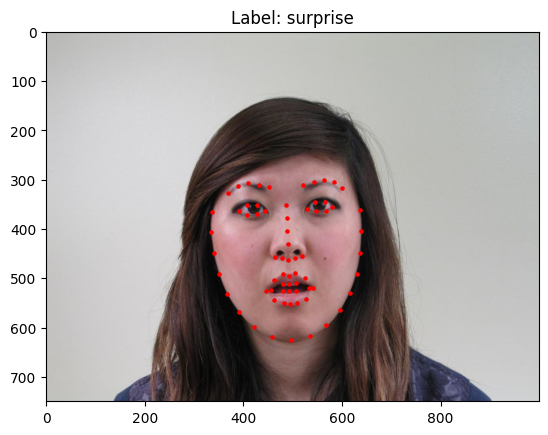
\includegraphics[height=6cm]{IMAGES/exemple1_landmark_jeu_donnee.png}
    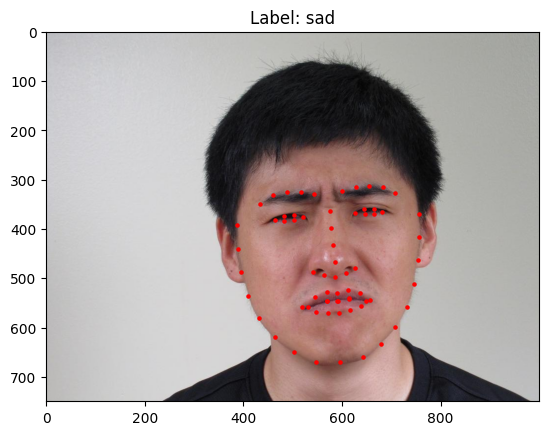
\includegraphics[height=6cm]{IMAGES/exemple2_landmark_jeu_donnee.png}
    \caption{Exemple de visage avec points clés}
    \label{fig:face_landmarks}
\end{figure}

\section{Prétraitement et Extraction des Features}
\subsection{Dans le cas des points de repères 2D}
Comme spécifié auparavant, nous disposons donc des 138 caractéristiques représentant les coordonnées des points repères du visage.
Avant de pouvoir construire notre modèle, il est essentiel de normaliser ces données.
Nous les normalisons donc selon la manière suivante \cite{kalapalaFacialExpressionRecognition2020} :\\

\begin{equation}
    X = \frac{(X - Xmean)} {Xstd}
\end{equation}\\

En parallèle, nous devons également appliquer un traitement sur les labels des données.
En effet ceux-ci correspondent à une variable qualitative parmi les 7 émotions.
Nous devons donc l'encoder en entier entre 0 et 6, chaque entier correspondant à une émotion en particulier.
Une fois ces traitements appliqués, nous pouvons commencer à réfléchir au modèle à utiliser.\\

\subsection{Dans le cas des images}
Nous avons également tenter de travailler avec les images.
En effet, les repères de visage présentent tout de même plusieurs inconvénients et une partie de l'information est perdue.
Les images quant à elle permettent d'avoir les textures,
les rides du visage et autres informations susceptibles d'aider dans la reconnaissance d'émotions.
Néanmoins, de nouveau défis surviennent lorsque nous utilisons les images, comme la luminosité ou encore l'orientation du visage.

Avant de les passer dans notre modèle, nous devons dans un premier temps appliquer plusieurs
traitements sur nos images. Étant donné qu'une grande partie de l'image n'est pas utile pour le modèle
(les cheveux, le cou, le fond de couleur grise) \ref*{fig:face_landmarks}, nous devons recadrer l'image
pour ne garder que le visage. Nous avons donc utiliser les points de repères pour recadrer l'image et
ne garder que le visage. Nous avons également redimensionné les images pour qu'elles aient toutes la même taille (96x96).
Le jeu de données étant assez petit, nous avons décidé de l'augmenter en utilisant différents procédés comme la
rotation selon un angle aléatoire entre -5° et 5° et le décalage horizontal avec une probabilité de 50\% \ref*{fig: exemple_image_augmentee}.
Ces méthodes permettent non seulement d'augmenter le jeu de données mais également de rendre le modèle plus général
et éviter le surapprentissage.

\insererfigure{IMAGES/images_normalized.png}{3cm}{Exemple d'image augmentée}{exemple_image_augmentee}

\section{Modèle(s) choisi(s)}
\subsection{Paramétrage et Entraînement}

\subsubsection{Dans le cas des points de repères 2D}
L'utilisation d'un modèle Support Vector Machine (SVM) n'est pas nouvelle est a déjà prouvé ses performances dans la reconnaissance
d'émotions \cite{kalapalaFacialExpressionRecognition2020}. Nous avons donc décidé d'utiliser ce modèle couplé à une GridSearch
afin de trouver les hyperparamètres optimaux pour le modèle.\\

GridSearch est une méthode utilisée afin de trouver les hyperparamètres optimaux
pour un modèle. Elle prend en paramètre une grille d'hyperparamètres et va tester en-
suite chaque combinaison pour faire ressortir la meilleure d'entre elle. Pour vérifier la
performance des paramètres, GridSearch utilise la méthode "k-fold cross-validation" qui
consiste à diviser les données d'entraînement en plusieurs sous-ensemble. Le modèle est
entraîné ensuite sur l'un de ces sous-ensemble et est évalué sur le reste des données. Ce
processus est répété k fois et permet d'éviter le surapprentissage du modèle. La meilleure
combinaison d'hyperparamètres est ensuite utilisée pour entraîner le modèle sur l'ensemble
des données d'entraînement. Il est important de noter que même si cette méthode permet
de trouver les hyperparamètres optimaux, elle reste tout de même très gourmande en
temps et en ressources\\

Nous avons donc décidé d'utiliser cette méthode afin d'obtenir les meilleurs hyperparamètres pour le modèle SVM. Il possède plusieurs paramètres :\\
\\- C aussi appelé paramètre de régularisation qui permet de gérer la marge. Une grande valeur de C implique une petite marge mais peu d'erreurs de classification
tandis qu'une petite valeur de C entraîne davantage d'erreur de classification mais une marge plus grande qui implique une plus grande généralisation.\\
- Le kernel qui permet de séparer les données. Nous pouvons choisir ici parmi plusieurs kernel dont 'rbf', 'linear' ou encore
'poly' ou 'sigmoid'.\\
- Gamma qui est un paramètre uniquement présent pour les kernels non-linéaires et qui permet d'épouser davantage la "forme" des données

Les résultats fournies par la GridSearch nous donnent les hyperparamètres optimaux pour notre modèle SVM. Nous trouvons
que le modèle SVM avec un kernel 'linear', un C de 10 et un gamma de 0.01 est le meilleur modèle pour notre jeu de données.\\

\subsubsection{Dans le cas des images}
Pour les images, nous avons décidé d'utiliser un modèle de réseau de neurones convolutif (CNN). Ces modèles ont démontrés
leur efficacité dans la reconnaissance d'images et notamment dans la reconnaissance d'émotions. La structure du modèle est la suivante :\\

\subsection{Résultats}

\subsubsection{Dans le cas des points de repères 2D}

Le meilleur modèle SVM entraîné sur les données fournies présente une précision de 78.06\% sur les données de tests. La matrice de confusion est présentée
sur la figure \ref*{fig:matrice_confusion_resultats}. Nous pouvons voir que le modèle a quelques difficultés à distinguer
et différencier les émotions 'anger' et 'disgust'. Ceci s'explique par le fait que ces deux émotions rendent le visage plutôt similaire avec
des poits clés du visage proches.\\

\insererfigure{IMAGES/matrice_confusion_resultats.png}{10cm}{Matrice de confusion des résultats}{matrice_confusion_resultats}


\subsubsection{Dans le cas des images}
Le modèle CNN entraîné sur les images augmentées et redimensionnées grâce aux points de repères du visage présente une précision
de 74.32\% sur les données de tests. Le graphique présentant l'évolution de la précision au cours de l'entraînement
sur les jeux de données d'entraînement et de validation est présentté sur la figure. Nous remaqruons qu'au bout d'un certain temps, la précision
en validation stagne tandis que celle en entraînement continue d'augmenter. Cela est sans doute dû à un surapprentissage du modèle.

\insererfigure{IMAGES/train_validation_acc.png}{8cm}{Précision du modèle CNN au cours de l'entraînement}{precision_cnn}

\section{Évaluation des Modèles}
\subsection{Discussions et Limites}

Le modèle SVM s'est montré plutôt performant avec les paramètres que nous avons choisis. Néanmoins, la précision du modèle est sujette à une certaine limite causée
majoritairement par le type et la forme des données en entrée du modèle. En effet, les points clés du visage ne sont pas forcément toujours caractéristique d'une émotion
et les points peuvent beaucoup varier d'une personne à l'autre quand bien même l'émotion représentée est la même. Les points repères du visage sont donc parfois biaisés selon
l'origine de la personne ou la forme de son visage. Nous pouvons cependant retenir que ce modèle présente un temps computationel plutôt court, notamment grâce au nombre réduit
de caractéristiques en entrée.\\
Lors du rapport intermédiaire et suite à une pseudo-labellisation manuelle des données de tests fournies, le modèle SVM obtient une précision de 52\%.
Cette précision est bien inférieure à celle reléve sur nos données de tests. Nous ne comprenons pas pourquoi cette différence est si importante.

\section{Conclusion}
Ce rapport a présenté différentes technique de Machine Learning pour la reconnaissance des émotions.
Nous avons abordé l'utilisation des points de repères du visage pour extraire les caractéristiques du visage et entraîner un modèle SVM.
Cette approche, bien que rapide et efficace, présente des limites en termes de généralisation et de précision. Les points clés du visage,
bien que représentatifs des émotions, peuvent varier d'une personne à l'autre et ne sont pas toujours caractéristiques d'une émotion.
Nous perdons également un certain nombre d'information comme les textures du visage ou encore les rides provoquées par l'émotion.
Les résultats montrent que l'utilisation des points de repères seuls ne suffisent pas pour une reconnaissance précise des émotions.
L'utilisation d'images couplée à celle des points de repère semble être une alternative solide comme le montre nos résultats. Néanmoins, nous
trouvons que la précision du modèle CNN est encore trop faible et que le modèle est sujet à un surapprentissage.


\bibliographystyle{ieeetr}
\bibliography{MLChallenge.bib}

\end{document}